\documentclass{beamer}
\usepackage{lmodern}
\usepackage{tikz}
\usetikzlibrary{decorations.pathmorphing}

\tikzset{snake it/.style={decorate, decoration=snake}}

\begin{document}


\begin{figure}
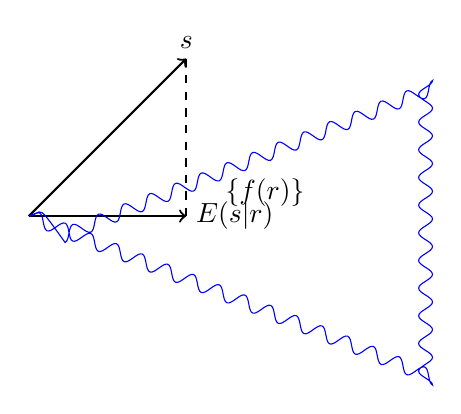
\begin{tikzpicture}
\draw [->, thick] (0,0) -- (2,2);
\draw [->, thick] (0,0) -- (2,0);
\path [draw=blue,snake it] (0,0) -- (5,-2) -- (5,2) -- (0,0);
\draw [dashed, thick] (2,2) -- (2,0);
\node [above] at (2,2) {$s$};
\node [right] at (2,0) {$E(s|r)$};
\node [above] at (3,0) {$\{f(r)\}$};
\end{tikzpicture}
\end{figure}

\end{document}